\section{Experimental Evaluation}
\label{sec:eval}
We ask whether the adaptation (i) enables complete DLA placement, (ii) provides
useful detection accuracy, and (iii) changes engine and application costs.
Evidence is separated by provenance: raw build/timing artifacts support the
placement and engine results; an embedded training history supports the
checkpoint metrics; a consolidated experiment summary provides provisional
application measurements. These sources do not offer equal validation.

\subsection{Platform, Artifacts, and Timing Protocol}
\label{sec:setup}
The device logs identify an NVIDIA Orin, compute capability 8.7, 16 streaming
multiprocessors, and 62,840\,MiB of reported device memory. TensorRT reports
version 10.3.0; strict execution targets DLA core 0. These properties are
recorded directly, but they do not uniquely establish the carrier configuration
or active operating conditions.
\missing{P1}{record exact module/carrier, JetPack/L4T, CUDA, power mode,
clock policy, temperatures, and matching artifact hashes}.

All engine comparisons enable FP16, with batch one and $640\times640$ inputs.
TensorRT may retain FP32 intermediates in GPU/fallback regions; this flag is
not a guarantee that every operation executes in FP16. The strict engine's
external bindings are FP16.
Each configuration has one \texttt{trtexec} launch with a 2\,s warm-up, a 30\,s
timing interval, one inference stream, spin waiting, generated input data, and
transfers enabled. The logged latency is
\begin{equation}
 L_{\mathrm{engine+IO}} = T_{\mathrm{H2D}}+T_{\mathrm{device}}+T_{\mathrm{D2H}}.
 \label{eq:latency}
\end{equation}
It excludes preprocessing, external decode, and NMS. On a DLA engine,
TensorRT's field named ``GPU Compute Time'' measures the device-execution
interval and does not prove GPU computation. Saturated throughput is completed
queries divided by host wall time; overlapping transfer and execution means
it need not equal the reciprocal of median latency.

The four retained timing traces contain 8,651 stock-GPU, 9,519 adapted-GPU,
878 stock-fallback, and 1,119 strict-DLA samples, matching the logged timed
counts. These are within-launch samples, not independent experimental repeats.
Reported P95 values describe those traces; they are not confidence intervals
on performance across launches or boards. Layer profiles were collected in
separate runs and are interpreted separately from transfer-inclusive timing.

\subsection{Fallback-Free Placement}
\label{sec:placement}
Stock YOLO11n fails strict compilation at its attention MatMul. The adapted
artifact compiles successfully; its build report assigns 299 layers to DLA and
reports no layers on the GPU. The optimized inspector represents the learned
graph as exactly one DLA layer with the three raw prediction outputs. Together,
the fallback-disabled build and inspector satisfy Eq.~\eqref{eq:accept} for
the recorded configuration.

The stock model with GPU fallback enabled produces a different result.
Its pre-optimization placement report assigns 317 layers to DLA and 17 to the
GPU. After optimization, the inspector contains four DLA loadables, eleven GPU
compute nodes, twenty-two reformat nodes, and ten no-op/constant nodes.
Figure~\ref{fig:profile} groups the optimized nodes and their measured profile
time. This is a successful heterogeneous deployment, but it does not meet the
complete learned-graph placement objective.

\begin{figure}[t]
\centering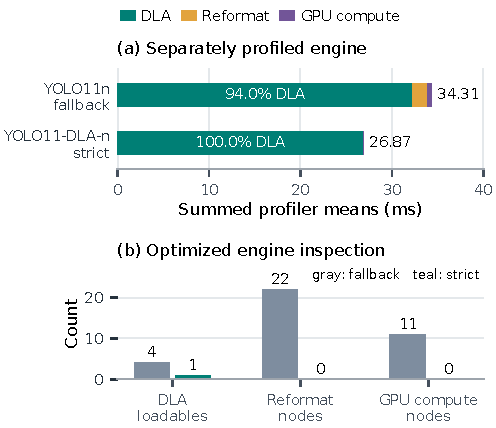
\includegraphics[width=\columnwidth]{figures/fallback_profile.pdf}
\caption{Stock YOLO11n with GPU fallback and the adapted strict-DLA engine.
Node counts come from engine inspection; time shares and summed means come
from separate layer-profile runs. DLA dominates the fallback engine's time
despite four loadables and intervening GPU/reformat work.}
\label{fig:profile}
\end{figure}

The four DLA loadables account for 93.97\% of profiled time, reformat nodes for
4.73\%, and GPU compute nodes for 1.30\%. The device profile totals about
34.312\,ms, including 32.244\,ms in DLA segments. These categories identify
where this compiled engine spends time. They do not isolate the causal cost of
partitioning: the strict graph also changes the attention computation and the
output interface. A matched-graph placement ablation is needed for that claim.

\subsection{Latency and Throughput at the Engine Boundary}
\label{sec:engine}
Table~\ref{tab:engine} reports the complete deployment matrix for YOLO11.
The strict adapted engine achieves 27.515\,ms median engine-plus-transfer
latency versus 34.678\,ms for stock YOLO11n with fallback. This is a 20.7\%
reduction, with throughput increasing from 29.2 to 37.2 queries/s (27.6\%).
Thus, the two graph changes enable complete DLA placement while improving
this engine-boundary comparison.

\begin{table}[t]
\caption{TensorRT FP16, batch one, $640\times640$. Latency includes transfers.
Each measured row is one launch; P95 is a within-launch percentile. Stock
strict DLA failed to build, so it has no timing result.}
\label{tab:engine}\centering\footnotesize
\setlength{\tabcolsep}{3pt}
\begin{tabular}{llrrr}
\toprule
Model & Device & Median & P95 & Rate \\
 & & (ms) & (ms) & (q/s) \\
\midrule
YOLO11n & GPU & 3.740 & 3.753 & 288.3 \\
YOLO11n & DLA+GPU & 34.678 & 34.942 & 29.2 \\
YOLO11n & Strict DLA & \multicolumn{3}{c}{Build rejected} \\
\model & GPU & 3.500 & 3.512 & 317.2 \\
\model & Strict DLA & 27.515 & 27.718 & 37.2 \\
\bottomrule
\end{tabular}
\end{table}

\begin{figure}[t]
\centering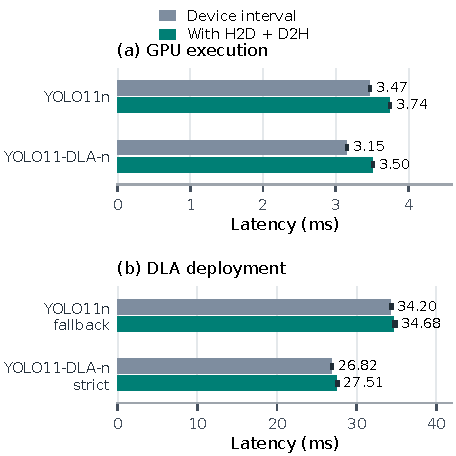
\includegraphics[width=\columnwidth]{figures/latency_comparison.pdf}
\caption{Device-execution and transfer-inclusive latency for the four successful
builds, with different horizontal scales for GPU and DLA panels. Medians and
P95 endpoints are computed from the retained timing traces;
the endpoints represent within-run variation. Device and total quantiles are
computed separately.}
\label{fig:latency}
\end{figure}

Figure~\ref{fig:latency} also exposes the cost of choosing DLA over the GPU.
The adapted model's GPU engine has a 3.500\,ms median, making its strict-DLA
execution 7.86 times slower. Relative to stock YOLO11n on the GPU, the ratio is
7.36. Median strict-DLA device execution is approximately 26.816\,ms; transfers
are a small component of this microbenchmark. This observation applies to the
measured engine and does not imply that its execution time is an unavoidable
lower bound for other compiler configurations or model variants.

The adapted GPU engine is slightly faster than the stock GPU engine, but their
output boundaries differ. Removing in-engine decode and modifying attention
both affect the comparison. We therefore use the adapted GPU row primarily as
a same-model execution control. Neither its engine timing nor the stock-fallback
comparison establishes complete-pipeline superiority.

\subsection{Accuracy Evidence and Training Record}
\label{sec:accuracy}
The retained adapted checkpoint embeds 500 epochs of training validation.
Table~\ref{tab:accuracy} reports its stored final metrics and
Fig.~\ref{fig:training} plots the retained history. The final AP is 37.581,
and AP$_{50}$ is 53.151, on the checkpoint's configured COCO validation task
\cite{lin2014coco}. These are checkpoint-recorded metrics, not a new independent
validation run. Stored validation precision and recall are 65.034\% and 48.557\%.

\begin{table}[t]
\caption{Accuracy provenance. AP is COCO AP averaged over IoU thresholds
0.50:0.05:0.95, in percentage points. Missing values are not inferred from model
names or literature benchmarks.}
\label{tab:accuracy}\centering\footnotesize
\setlength{\tabcolsep}{3pt}
\begin{tabular}{p{.40\columnwidth}ccp{.21\columnwidth}}
\toprule
Model / evaluation & AP & AP$_{50}$ & Evidence \\
\midrule
\model / training validation & 37.581 & 53.151 & Stored epoch 500 \\
YOLO11n / matched PyTorch & \missing{P2}{AP} & \missing{P2}{AP} & Pending \\
\model / independent PyTorch & \missing{P2}{AP} & \missing{P2}{AP} & Pending \\
\model / strict DLA & \missing{P3}{AP} & \missing{P3}{AP} & Pending \\
\bottomrule
\end{tabular}
\end{table}

\begin{figure}[t]
\centering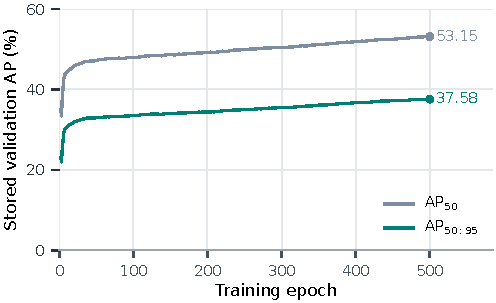
\includegraphics[width=\columnwidth]{figures/training_history.pdf}
\caption{Validation history embedded in the retained \model{} checkpoint.
This is one recorded 500-epoch training run, without repeated-seed uncertainty
or a paired stock-YOLO11n training curve. It is not serialized-engine accuracy.}
\label{fig:training}
\end{figure}

A paired reference evaluation under identical preprocessing and evaluator
settings is absent. Accordingly, no measured accuracy-retention percentage or
accuracy-loss claim is made. The exported ONNX and engines also need a verified
identity chain back to the checkpoint, because filenames do not certify that
they contain the same weights. The remaining numerical test must distinguish
three effects: the changed architecture, export/FP16 arithmetic, and the native
runtime/decoder path.

\subsection{Local Export and Decoder Verification}
\label{sec:parity}
We additionally execute a reproducible CPU check on the retained checkpoint and
ONNX artifact, using one $1\times3\times640\times640$ uniform-random input
with seed 7. External dense decoding of the adapted PyTorch raw maps agrees
with the same model's ordinary decoded output: maximum absolute error is
$1.22\times10^{-4}$, and mean absolute error is $5.45\times10^{-8}$. The
elementwise comparison passes with relative tolerance $10^{-5}$ and absolute
tolerance $10^{-4}$; these tolerances are combined, not separate maximum-error
limits. The output has shape $1\times84\times8400$ before NMS.

ONNX Runtime CPU inference also agrees with the checkpoint's three raw outputs
under relative/absolute tolerances $10^{-4}/10^{-3}$. Maximum absolute errors
are $2.08\times10^{-4}$, $3.07\times10^{-4}$, and $6.87\times10^{-5}$ for
P3, P4, and P5. ONNX structural validation and the output-shape checks pass.
The script records artifact and input hashes plus library versions. These
checks exercise the export interface and dense decoder on one input; they
do not compare against stock YOLO11, certify sparse NMS equivalence, or execute
the serialized DLA engine.

\subsection{Application Measurements: Provisional Evidence}
\label{sec:application}
The experiment summary retains results from a sequential runner with ten warm-up
iterations and 100 timed repetitions of one $960\times1280$ image. It uses
CPU post-processing, confidence 0.25, and NMS IoU 0.45, excluding file reading,
drawing, and writing. The original YOLO11-family per-frame JSON records are not
present in the supplied log directory. Table~\ref{tab:e2e} is therefore
explicitly a transcription of summary-level evidence, pending recollection.

\begin{table}[t]
\caption{Provisional repeated-image pipeline medians in ms, transcribed from the
retained summary. I/O sums the pack/H2D and D2H/unpack stage medians. Medians need not
sum to median total. \missing{P4}{replace with raw multi-image results}.}
\label{tab:e2e}\centering\footnotesize
\setlength{\tabcolsep}{3pt}
\begin{tabular}{lrrrrr}
\toprule
Model / device & Pre & I/O & Engine & Post & Total \\
\midrule
11n / GPU & 4.900 & 2.843 & 8.153 & 3.250 & 19.203 \\
11n / DLA+GPU & 8.617 & 4.002 & 35.198 & 4.866 & 52.782 \\
11-DLA / GPU & 4.572 & 3.848 & 7.560 & 3.717 & 19.831 \\
11-DLA / DLA & 8.946 & 13.992 & 27.788 & 5.711 & 56.497 \\
\bottomrule
\end{tabular}
\end{table}

These preliminary totals reverse the engine-boundary ordering between strict
DLA and stock fallback: 56.497 versus 52.782\,ms. The sum of the strict path's
I/O stage medians is 13.992\,ms, including conversion and transfer; its host
decode is additional work relative to stock YOLO11n's decoded output. Different
preprocessing times for the same image and code also reveal uncontrolled
between-launch conditions. Without raw traces and platform telemetry, those
differences cannot be assigned to CPU clocks, thermals, or accelerator
contention. Summing or subtracting stage medians does not provide an exact
per-frame decomposition.

The summary reports matching classes and displayed confidences for the adapted
GPU and DLA paths, with at most 0.3 pixels difference in displayed box
coordinates on this image. This is a provisional smoke check, not dataset-level
numerical equivalence. No energy measurements or concurrent-task timing results
are present in the supplied evidence.
